\def\year{2017}\relax
\documentclass[letterpaper]{article}
\usepackage{aaai17}
\usepackage{times}
\usepackage{helvet}
\usepackage{courier}
\usepackage{graphicx}
\usepackage{url}  %Required
\usepackage{multirow}
\usepackage{subfig}
%\setlist{nosep} % dense lists with enumitem
 
\newcommand{\xmark}{\ding{55}}%
\newcommand{\starmark}{\ding{72}}%

%\renewcommand{\vec}[1]{\mathbf{#1}}  commented due to AAAI Formating

\newcommand{\eat}[1]{}
\newcommand{\rev}[1]{{\color{blue}{#1}}}


\frenchspacing
\setlength{\pdfpagewidth}{8.5in}
\setlength{\pdfpageheight}{11in}

%============================================================

\pdfinfo{
/Title (A Longitudinal Study of Topic Classification on Twitter)
/Author (Zahra Iman, Scott Sanner, Mohamed Reda Bouadjenek, Lexing Xie)}
\setcounter{secnumdepth}{1}  

 \begin{document}
% The file aaai.sty is the style file for AAAI Press 
% proceedings, working notes, and technical reports.
%
\title{A Longitudinal Study of Topic Classification on Twitter}
%\author{Authors\\
%Affiliations
%}
\author {Zahra Iman$^{\dag}$, Scott Sanner$^{\ddagger}$, Mohamed Reda Bouadjenek$^{*}$, Lexing Xie$^{\S}$\\
	$^{\dag}$Oregon State University, Corvallis, OR, USA\\
	$^{\ddagger}$University of Toronto, Toronto, ON, Canada\\
	$^{*}$University of Melbourne, Melbourne, VIC, Australia\\
	$^{\S}$Australian National University and Data61, Canberra, ACT, Australia\\
	%\{suvash.sedhain, aditya.menon\}@data61.csiro.au, ssanner@mie.utoronto.ca, lexing.xie@anu.edu.au, dbraziunas@kobo.com
	{\footnotesize zahra.iman87@gmail.com, ssanner@mie.utoronto.ca, reda.bouadjenek@unimelb.edu.au, lexing.xie@anu.edu.au}
}
\maketitle
\begin{abstract}
Twitter represents a massively distributed information source over a kaleidoscope of topics ranging from social and political events to entertainment and sports news.  While recent work has suggested that variations on standard classifiers can be effectively trained as topical filters~\cite{lin2011smoothing,yang2014large,magdy}, there remain many open questions about the efficacy of such classification-based filtering approaches.  For example, over a year or more after training, how well do such classifiers generalize to future novel topical content, and are such results stable across a range of topics?  Furthermore, what features and feature classes are most critical for long-term classifier performance?  To answer these questions, we collected a corpus of over 800 million English Tweets via the Twitter streaming API during 2013 and 2014 and learned topic classifiers for 10 diverse themes ranging from social issues to celebrity deaths to the ``Iran nuclear deal''.  The results of this long-term study of topic classifier performance provide a number of important insights, among them that (1)~such classifiers can indeed generalize to novel topical content with high precision over a year or more after training and (2)~simple terms and locations are the most informative feature classes (despite training on classes labeled via hashtags).
\end{abstract}

\section{Learning Topical Social Sensors}
\label{sec:lss}
Our objective is to evaluate binary classifiers that can label
a previously unseen tweet as topical (or not).
Following
the approach of~\cite{lin2011smoothing}, for a topic~$t$, we leverage a (small) set of
user-curated topical hashtags $H^t$ to efficiently provide a large number of
supervised topic labels for training.  
As standard for machine learning methods, we divide our training data into
train and validation sets --- the latter for hyperparameter tuning to control
overfitting and ensure generalization to unseen data.  
As a critical insight for topical generalization where we view correct classification 
of tweets with \emph{previously unseen topical hashtags} as a proxy for topical generalization, 
we \emph{do not} simply
split our data temporally into train, validation, and test sets and label both with \emph{all} 
hashtags in $H^t$.  \emph{Instead},
we split $H^t$ into three disjoint sets $H^t_\mathrm{train}$, $H^t_\mathrm{val}$, and 
$H^t_\mathrm{test}$ 
according to two time stamps $t^\mathrm{val}_\mathrm{split}$ and $t^\mathrm{test}_\mathrm{split}$ for topic $t$ and the first usage time stamp 
$h_\mathrm{time*}$ of each hashtag $h \in H^t$.  In short, all hashtags $h \in H^t$ with
$h_\mathrm{time*} < t^\mathrm{val}_\mathrm{split}$ are used to generate positive labels in the training data, those with $h_\mathrm{time*} \geq t^\mathrm{test}_\mathrm{split}$ are used for positive labels in the test data and the remainder are used for positive labels in the validation data.

The key point to observe is that we not only partition the train, validation, and test data 
temporally, but we also divide the hashtag class labels temporally and label each data partition with
an entirely disjoint set of topical hashtags.
The purpose behind this training and validation data split
and labeling is to ensure that learning hyperparameters are tuned so as
to prevent overfitting and maximize generalization to unseen topical
content (i.e., new hashtags).
We remark that a classifier that simply
memorizes training hashtags will fail to correctly classify the validation data except in 
cases where a tweet contains both a training and validation hashtag.

\section{Data Description}
\label{sec:datasetStatistics}
\begin{table}[t!]
\centering
{%\renewcommand{\arraystretch}{1.2}commented due to AAAI Formating
\resizebox{\columnwidth}{!}{%
\begin{tabular}{|c|c|c|c|c|}
%\hline
\multicolumn{5}{c}{\textbf{\#Unique Features}} \\ \hline
\textbf{From} & \textbf{Hashtag} & \textbf{Mention} & \textbf{Location} & \textbf{Term} \\ \hline
95,547,198 & 11,183,410 & 411,341,569 & 58,601 & 20,234,728 \\ \hline %14,197,509
\end{tabular}
}}
\resizebox{\columnwidth}{!}{%
\begin{tabular}{|l|c|c|c|c|}
%\hline
\multicolumn{5}{c}{} \\
\multicolumn{5}{c}{\textbf{Feature Usage in \#Tweets}} \\ \hline
\textbf{Feature} & \textbf{Max} & \textbf{Avg} & \textbf{Median} & \textbf{Most frequent} \\ \hline
\textbf{From} & 10,196 & 8.67 & 2 & running\_status \\ \hline
\textbf{Hashtag} & 1,653,159 & 13.91 & 1 & \#retweet \\ \hline
\textbf{Mention} & 6,291 & 1.26 & 1 & tweet\_all\_time \\ \hline %$\rightarrow$null \\ \hline
\textbf{Location} & 10,848,224 & 9,562.34 & 130 & london \\ \hline
\textbf{Term} & 241,896,559 & 492.37 & 1 & rt \\ \hline 
\multicolumn{5}{c}{} \\
\multicolumn{5}{c}{\textbf{Feature Usage by \#Users}} \\ \hline
\textbf{Hashtag} & 592,363 & 10.08 & 1 & \#retweet \\ \hline
\textbf{Mention} & 26,293 & 5.44 & 1 & dimensionist \\ \hline
\textbf{Location} & 739,120 & 641.5 & 2 & london \\ \hline
\textbf{Term} & 1,799,385 & 6,616.65 & 1 & rt \\ \hline %SHOULD BE FIXED
\multicolumn{5}{c}{} \\
\multicolumn{5}{c}{\textbf{Feature Using \#Hashtags}} \\ \hline
\textbf{From} & 18,167 & 2 & 0 & daily\_astrodata \\ \hline
\textbf{Location} & 2,440,969 & 1,837.79 & 21 & uk \\ \hline
\end{tabular}
}
\caption{Feature Statistics of our $829,026,458$ tweet corpus.} % in our Twitter dataset}
\label{table:featureStatistics}
\end{table}
%%%%%%%%%%%%%%%%%%%%%%%%%%%%%%%%%%%%%%%%%%%%%%%%%%%%%%%%%%%%%%%%%%
%%%%%%%%%%%%%%%%%%%%%%%%%%%%%%%%%%%%%%%%%%%%%%%%%%%%%%%%%%%%%%%%%%%%%%%%%%%
\begin{figure*}[t!]
\centering
\resizebox{\textwidth}{!}{
\begin{tabular}{ccc}
\subfloat[Fig:][Human Caused Disaster]{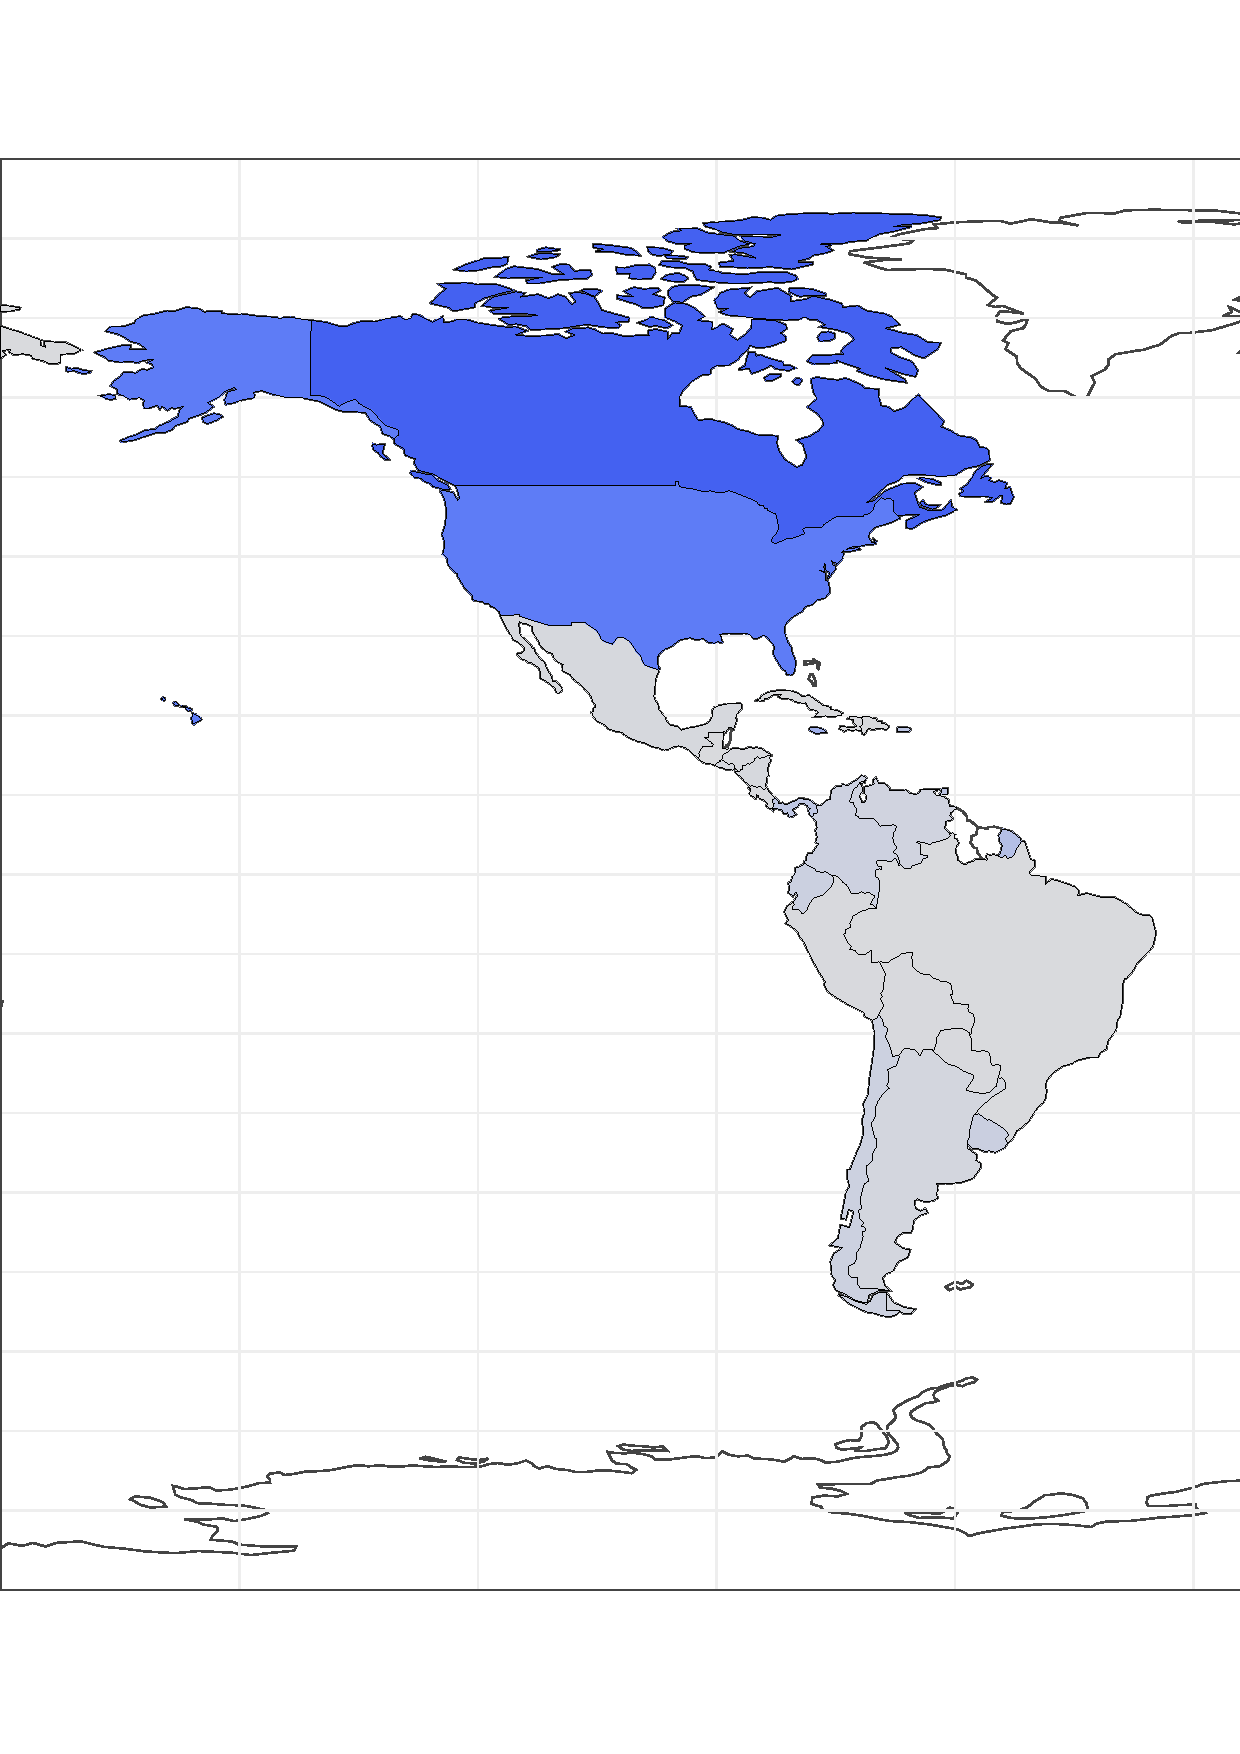
\includegraphics[width=0.33\textwidth]{images/location/world/socialsensor-world-HumanCausedDisaster_location.pdf}}
\subfloat[Fig:][Iran Deal]{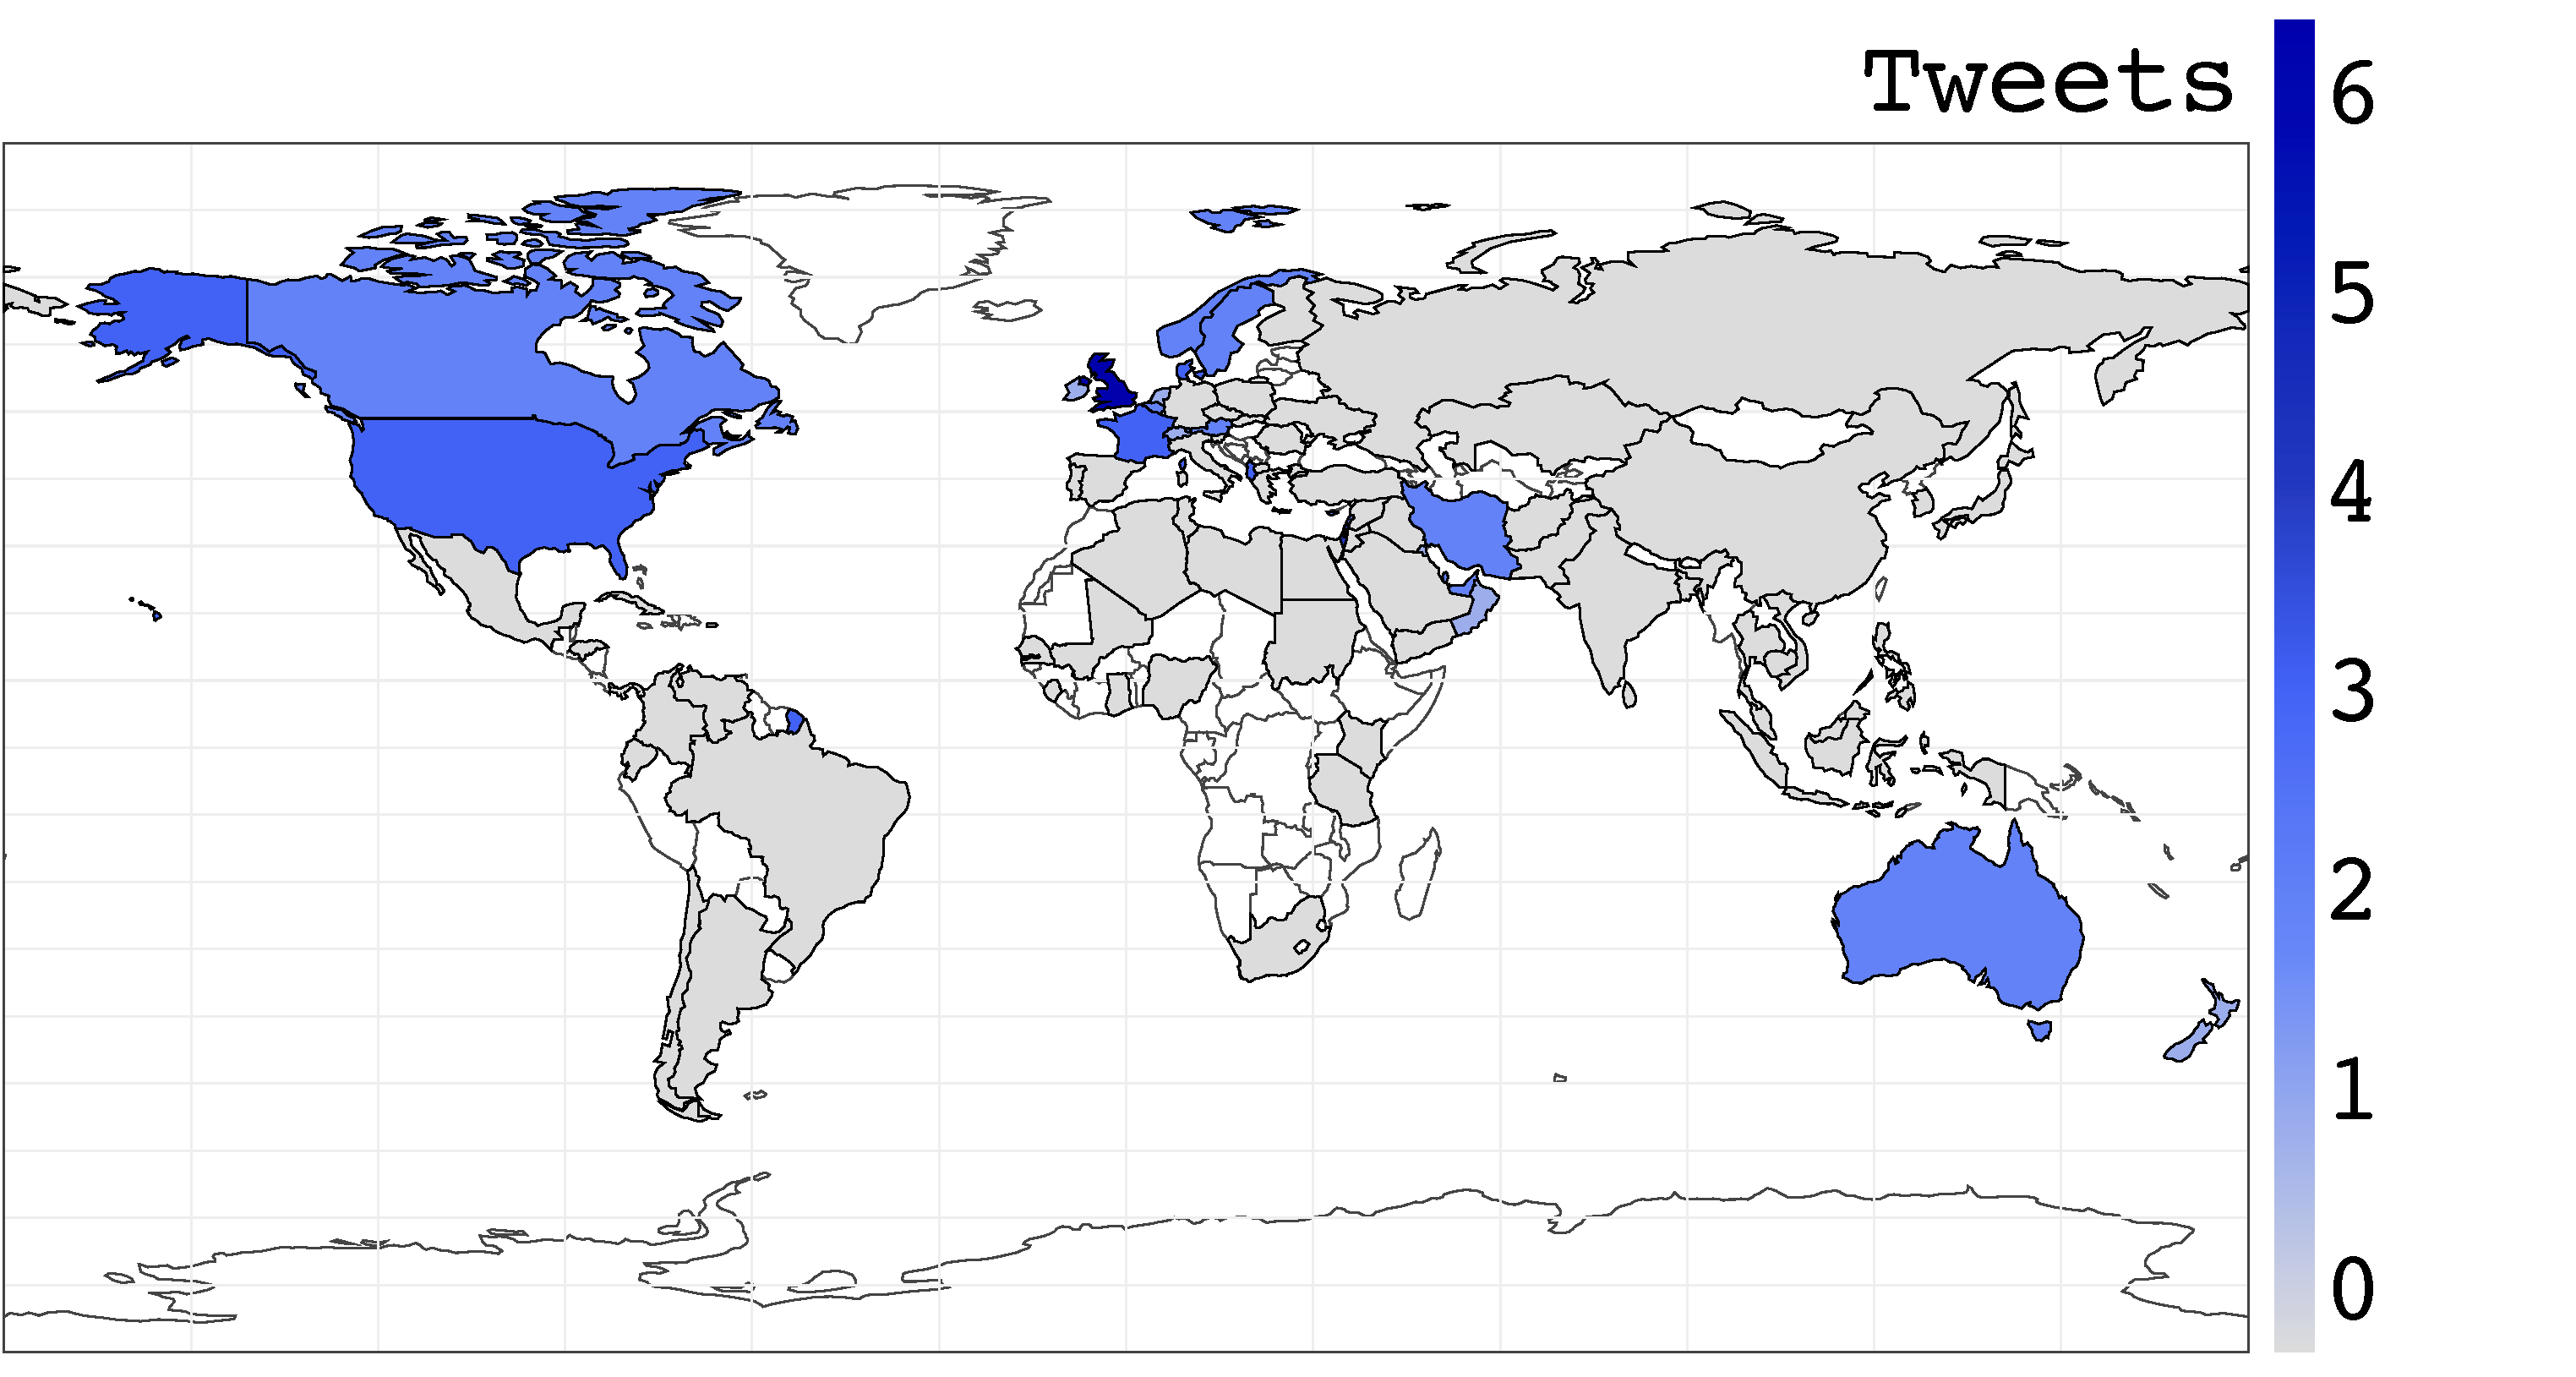
\includegraphics[width=0.33\textwidth]{images/location/world/socialsensor-world-irannucleardeal_location.pdf}}
\subfloat[Fig:][Soccer]{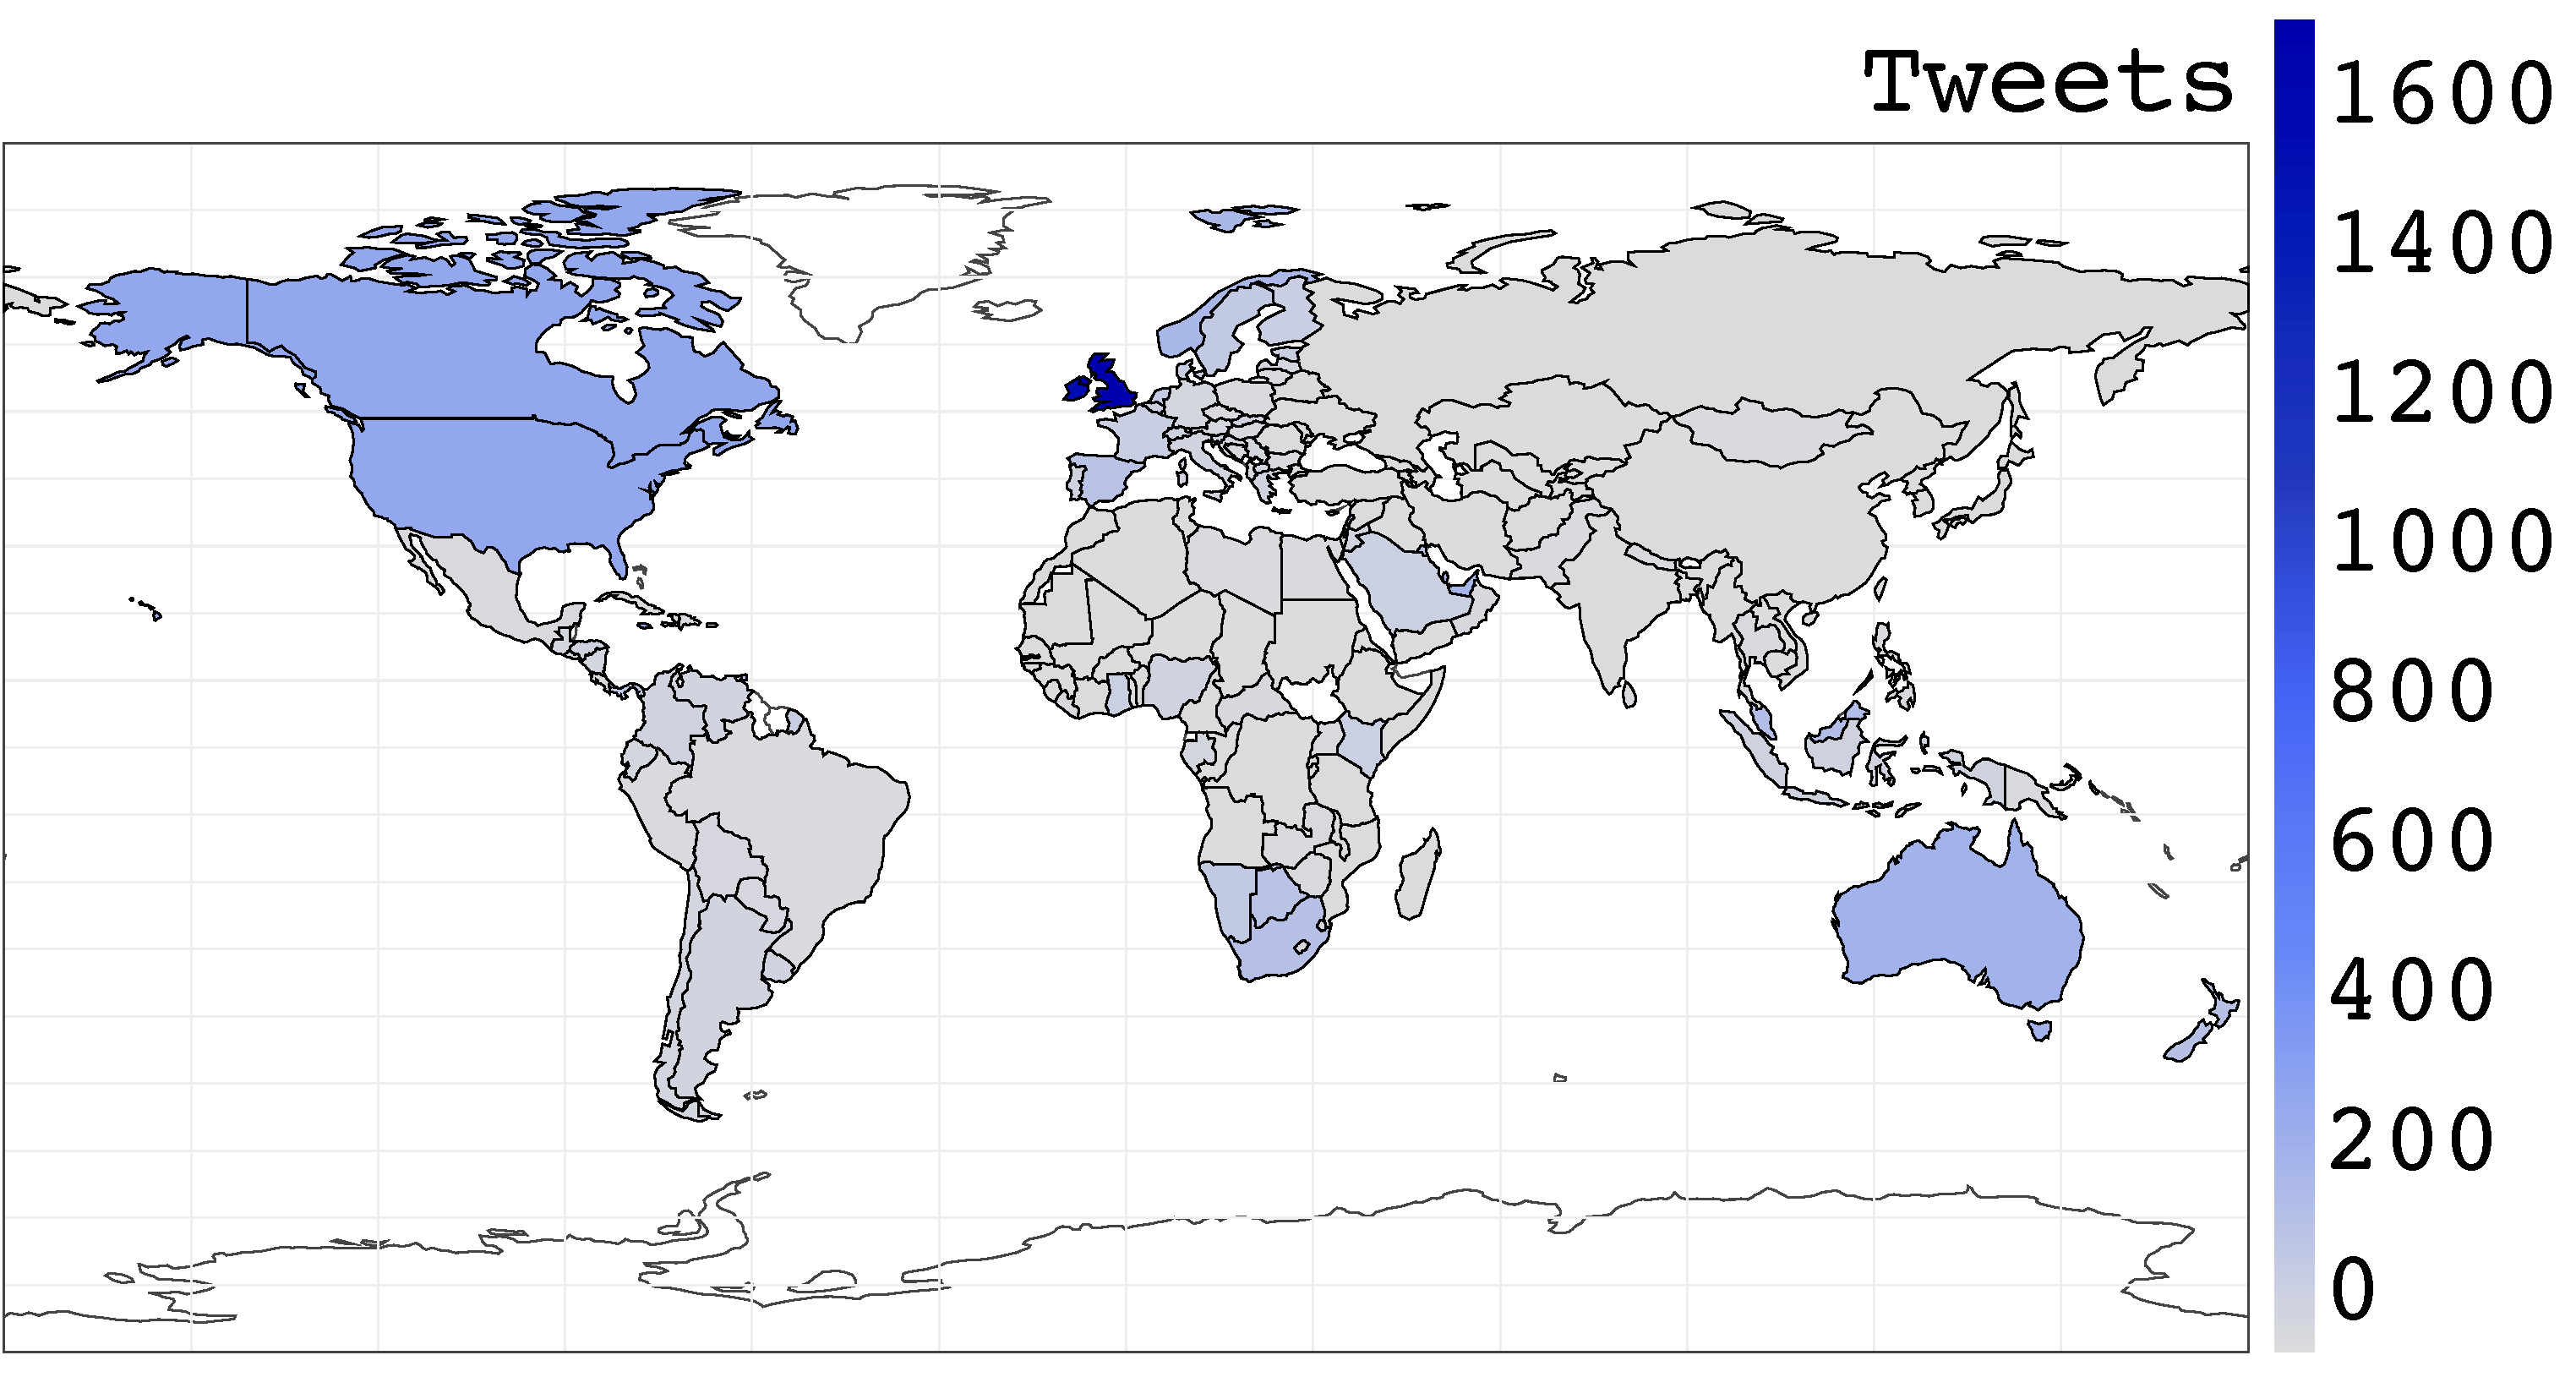
\includegraphics[width=0.33\textwidth]{images/location/world/socialsensor-world-soccer_location.pdf}} \\
\subfloat[Fig:][Health Epidemics]{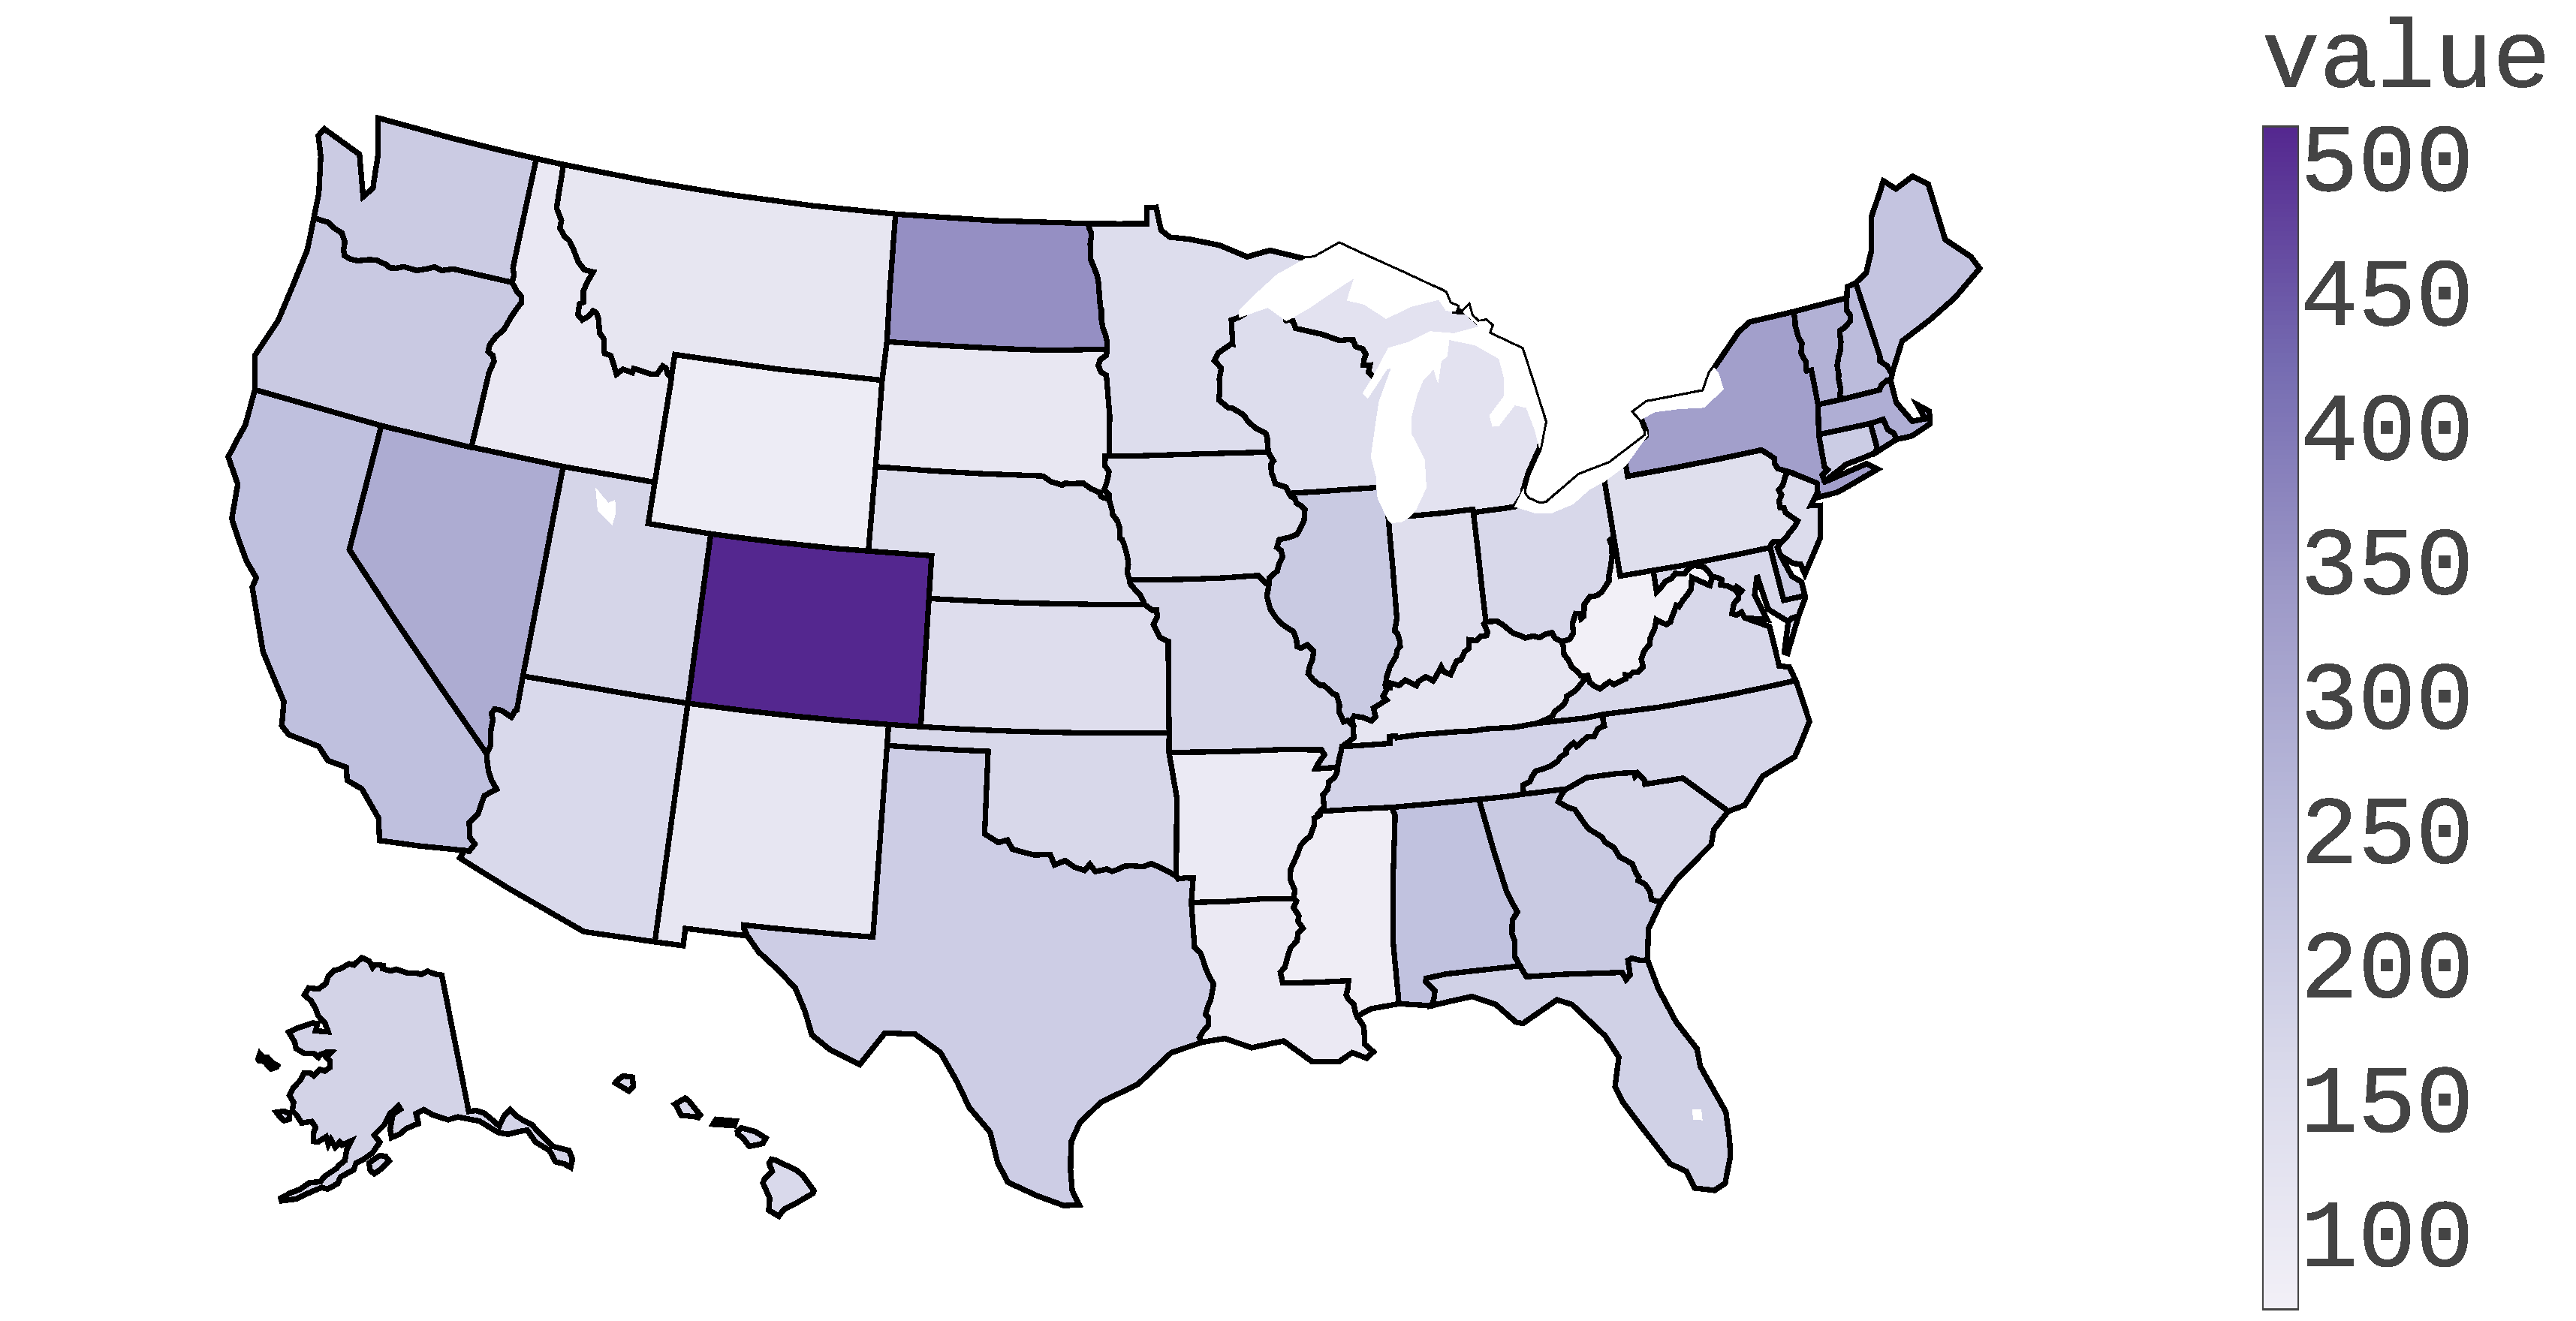
\includegraphics[width=0.33\textwidth]{images/location/states/SocialSensor-us-states-health_epidemics_location.pdf}}
\subfloat[Fig:][Social Issues]{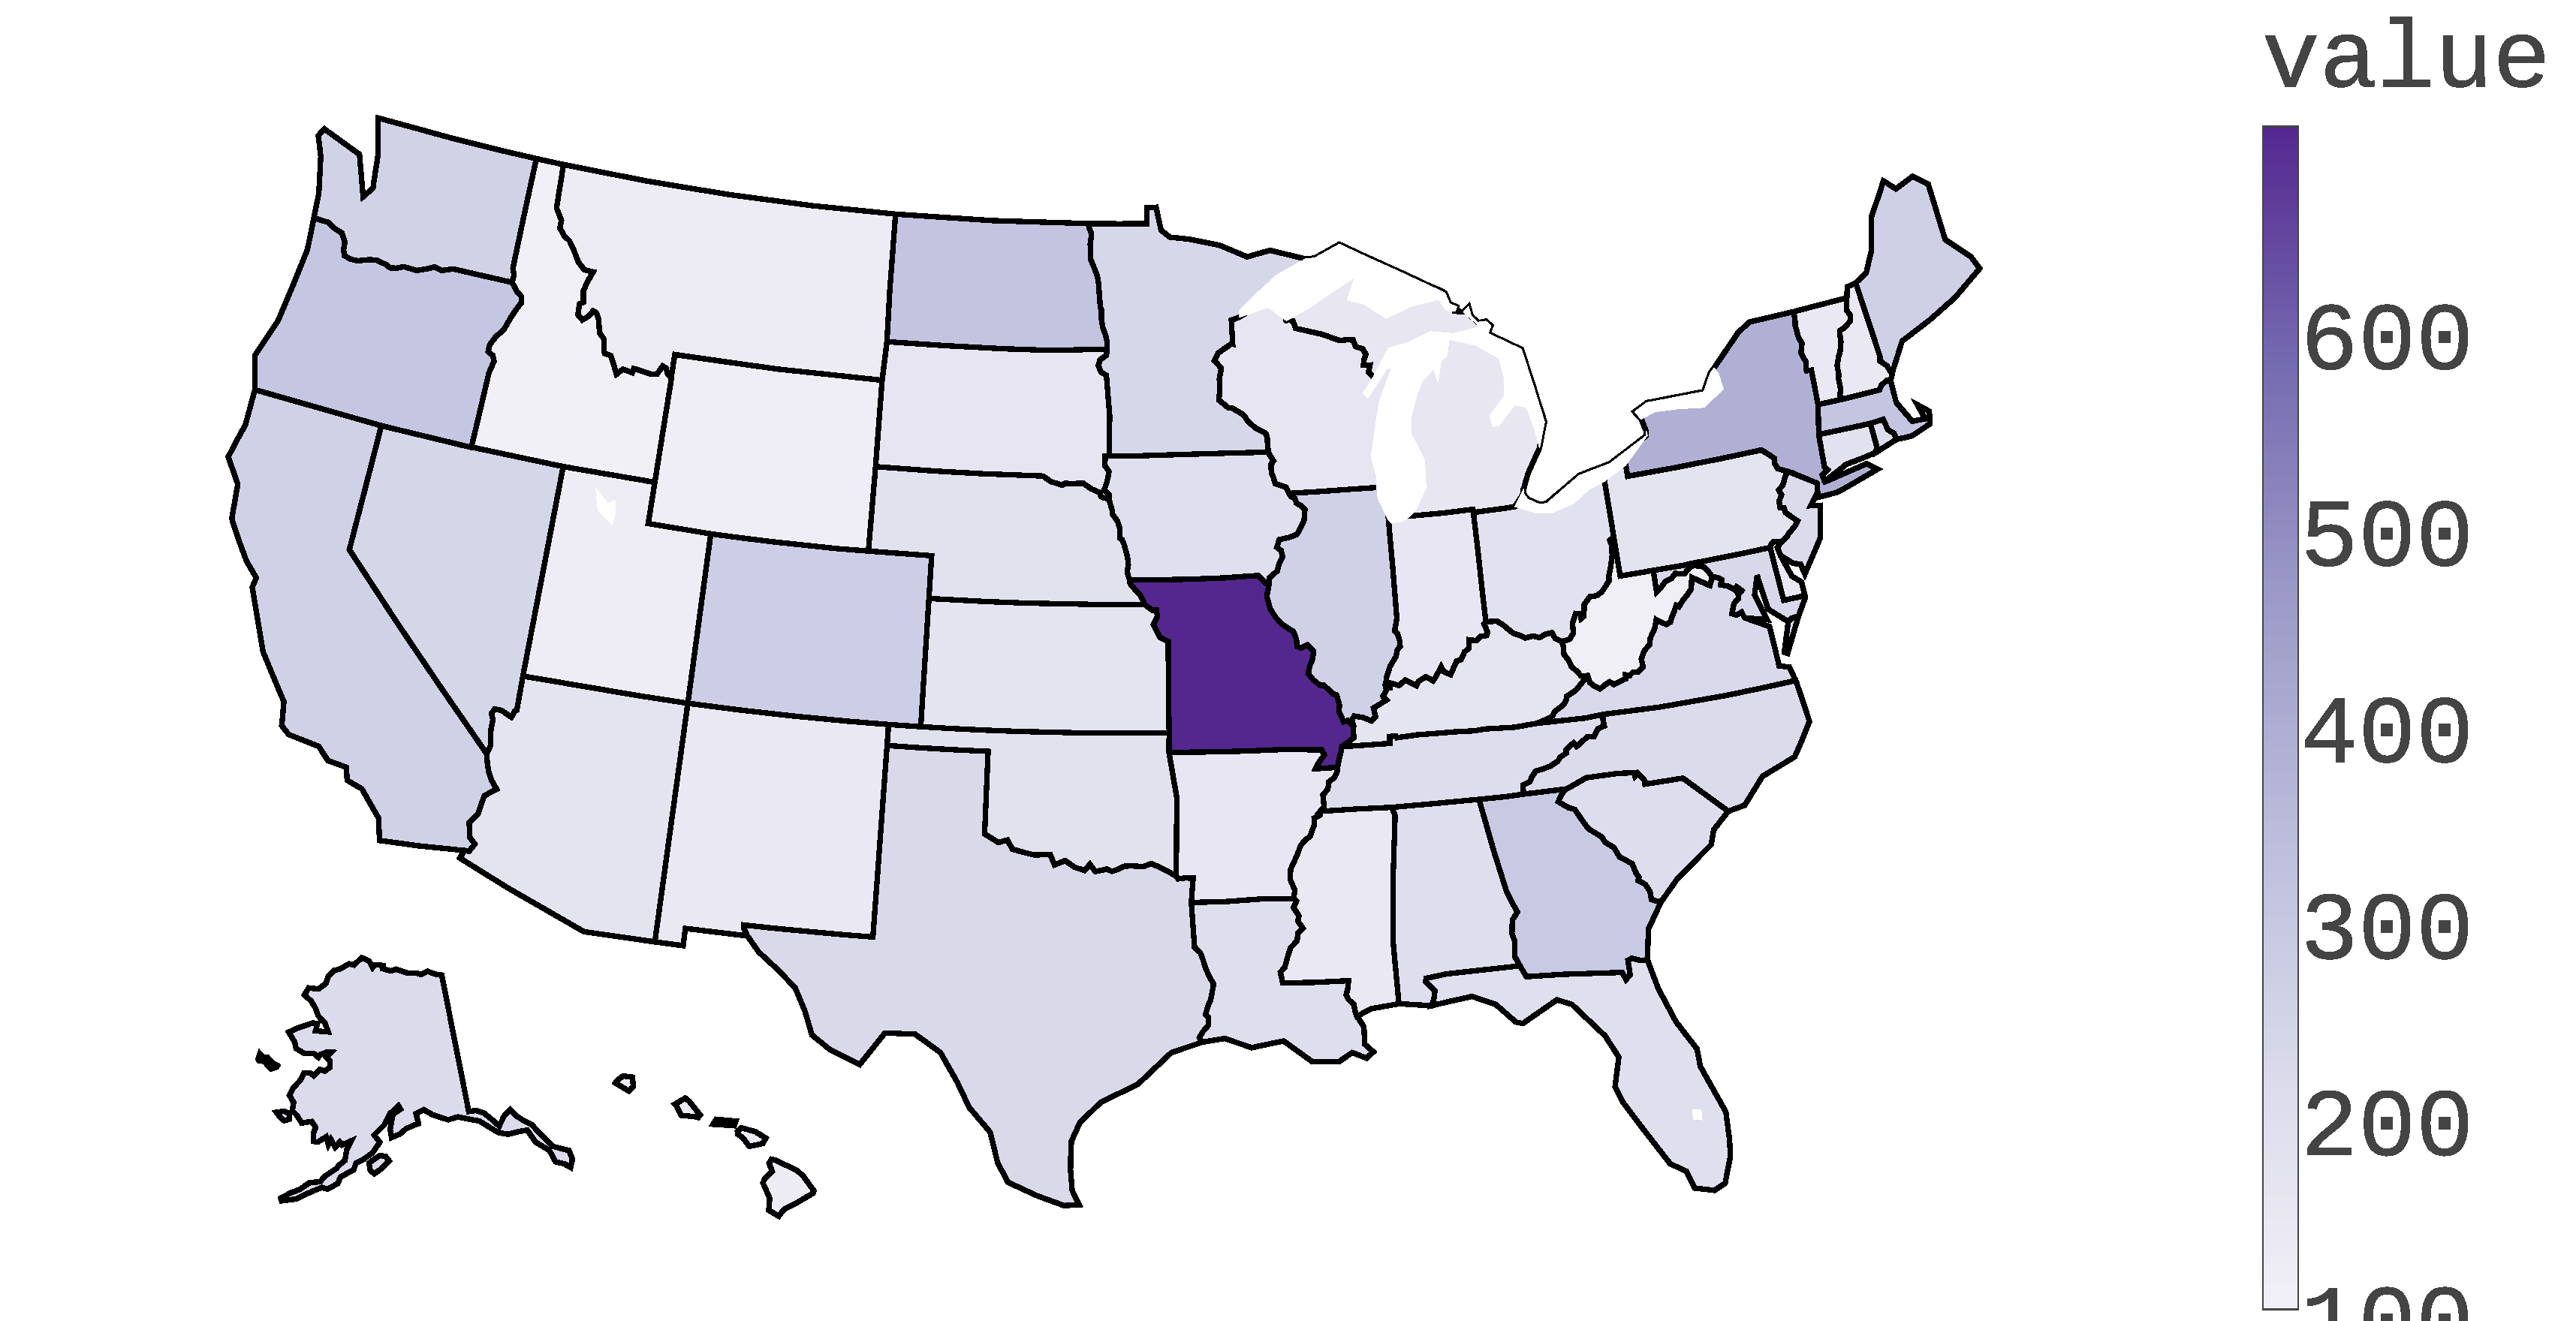
\includegraphics[width=0.33\textwidth]{images/location/states/SocialSensor-us-states-socialissues_location.pdf}}
\subfloat[Fig:][Space]{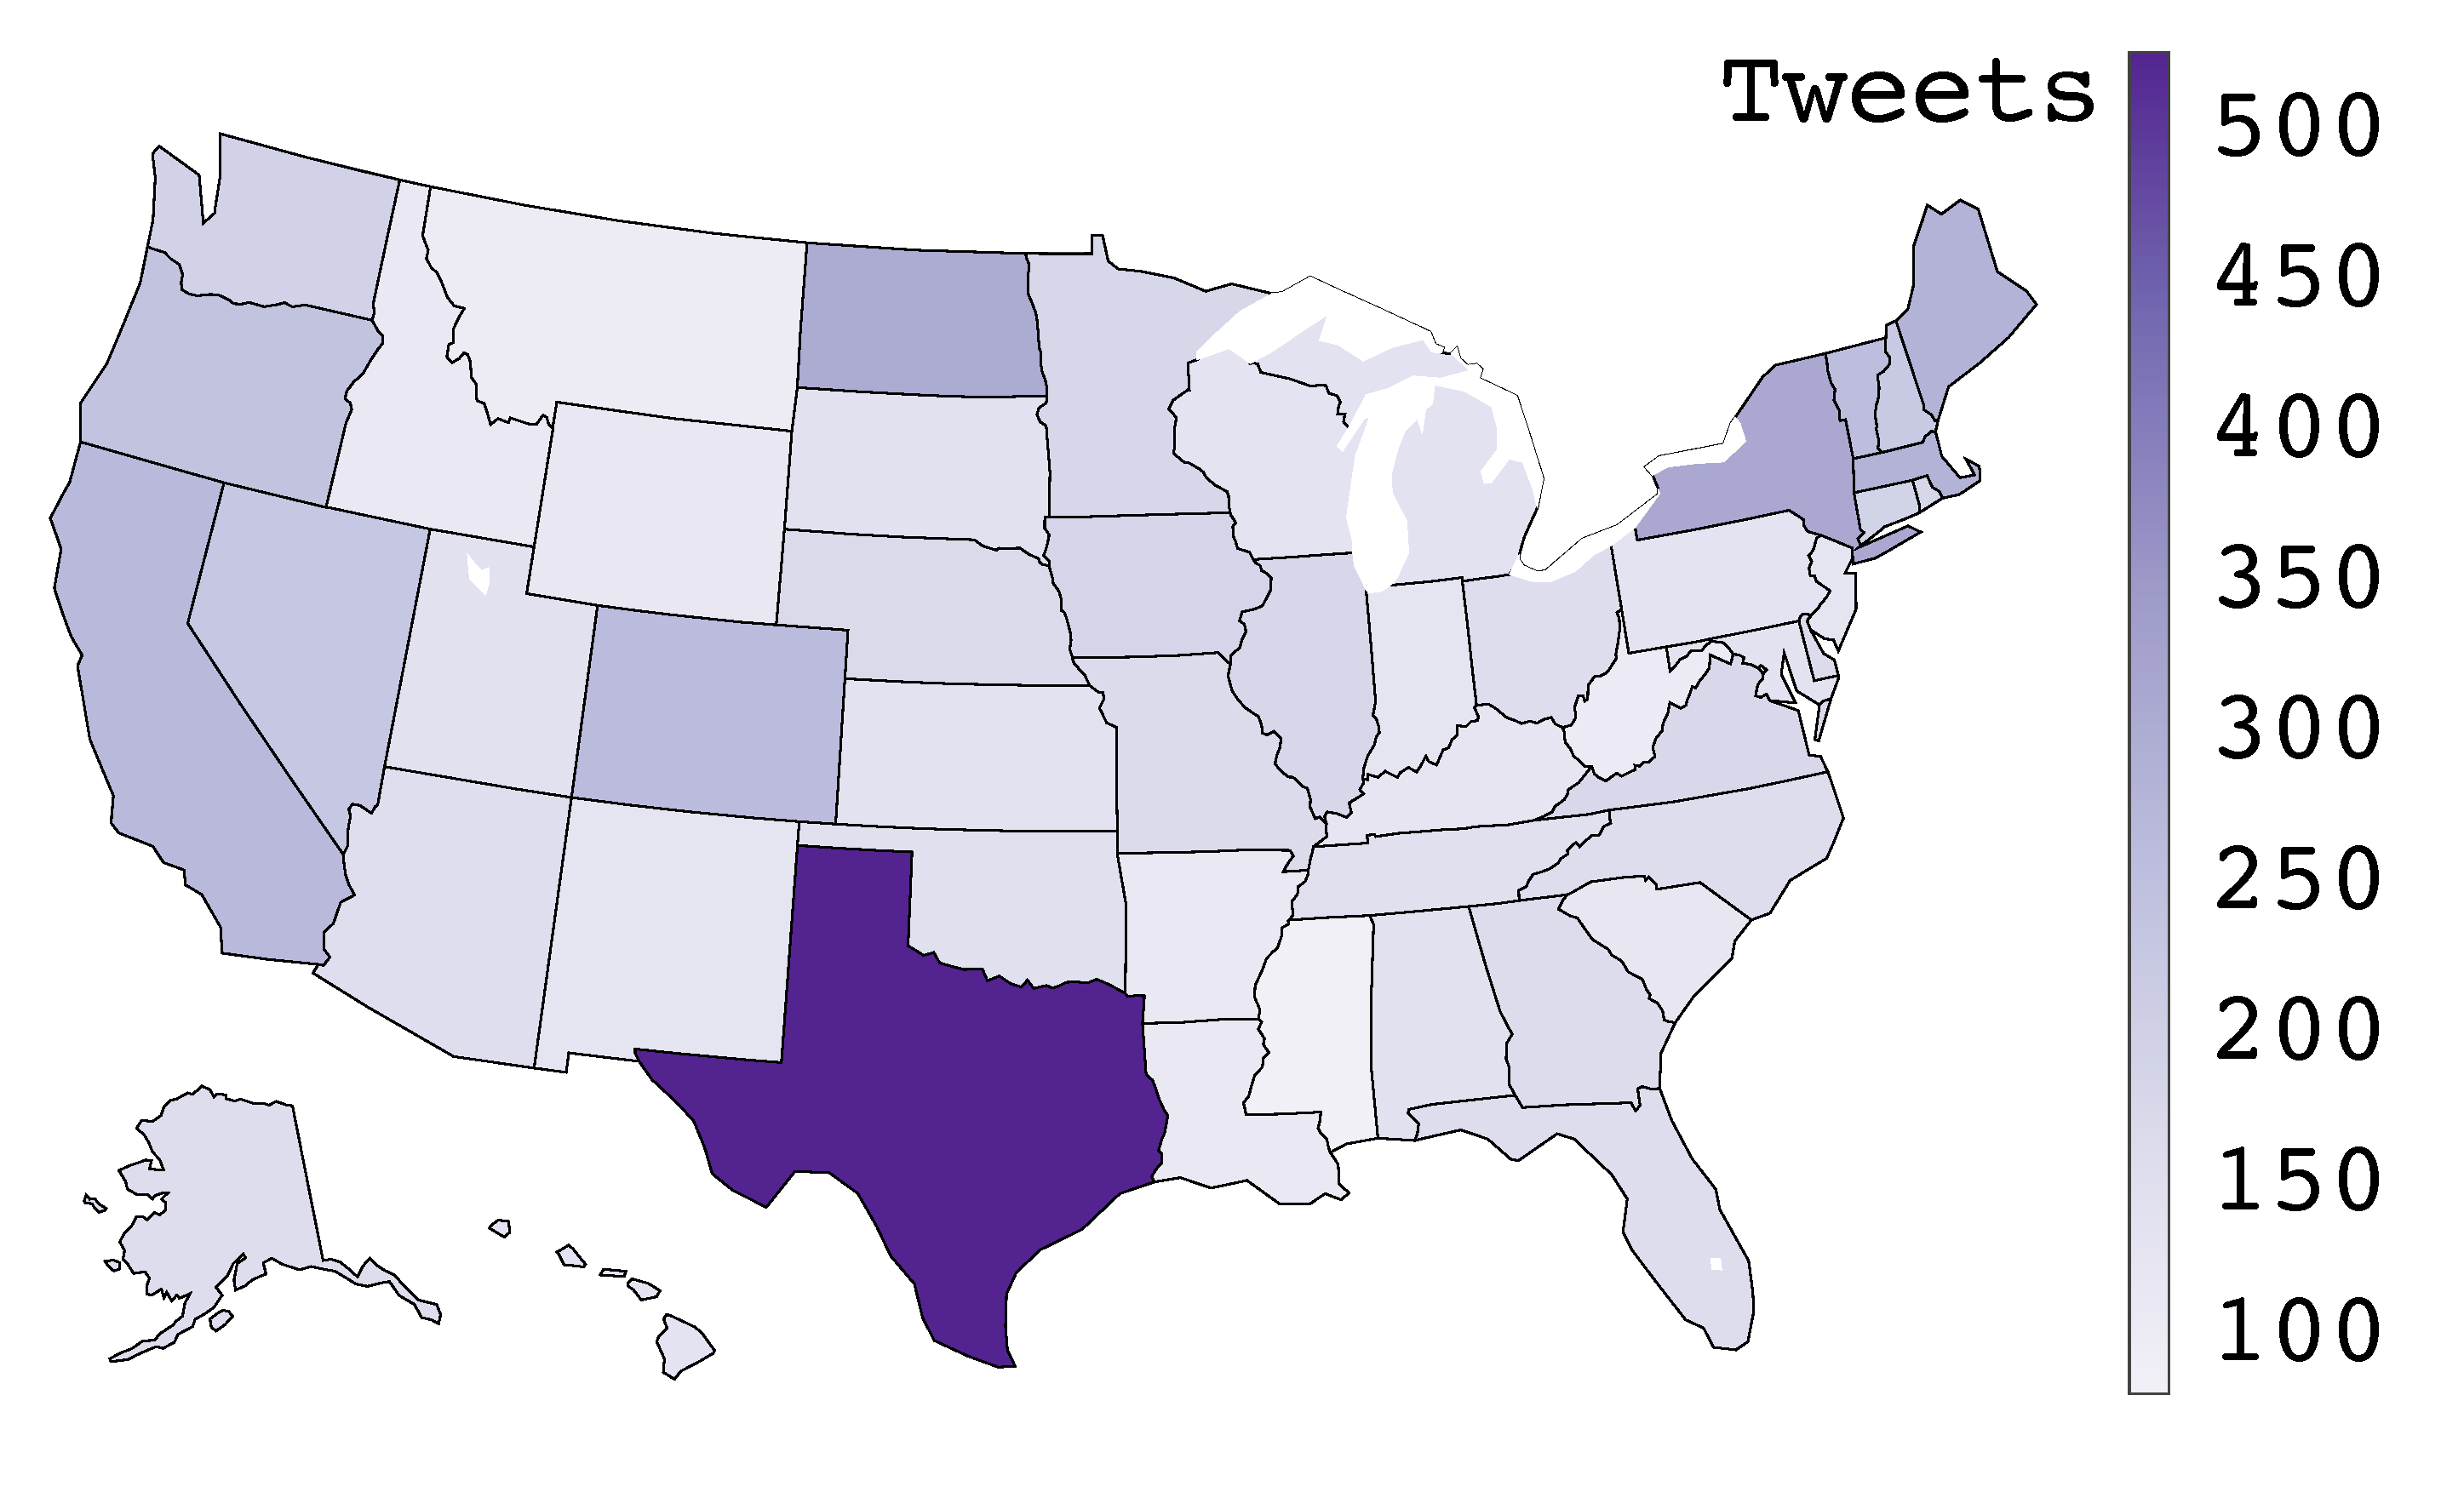
\includegraphics[width=0.33\textwidth]{images/location/states/SocialSensor-us-states-space_location.pdf}} \\
\end{tabular}
}
\caption {Tweets per 1 Million capita tweet frequency across different international and U.S. locations for different topics.}
\label{fig:choropleths}
\end{figure*}
%%%%%%%%%%%%%%%%%%%%%%%%%%%%%%%%%%%%%%%%%%%%%%%%%%%%%%%%%%%%%%%%%%%%%%%%%%%

We crawled Twitter data using the Twitter 
Streaming API for two years spanning 2013 and 2014.
We collected more than 2.5 TB of compressed data, which contains a total  
of $829,026,458$ English tweets. In the context 
of Twitter, we consider five feature types for each tweet.  Each
tweet has a \textit{From} feature (i.e., the person who tweeted it), a
possible \textit{Location} (i.e., a string provided as meta-data), and
a time stamp when it was posted.  A tweet can also contain one or more
of the following:
\textit{Hashtag} (i.e., a topical keyword specified using the \# sign), 
\textit{Mention} (i.e., a Twitter username reference using the @ sign), % reply?
\textit{Term} (i.e., any non-hashtag and non-mention unigrams). %These uni-grams are later cleaned to remove $Term$s with no meaning (total number of $Term$s before cleaning was $20,234,729$)
%\end{itemize}
We provide detailed feature statistics in Table~\ref{table:featureStatistics}.  

Fig.~\ref{fig:choropleths} shows per capita tweet frequency across
different international and U.S. locations for different topics.
While English speaking countries dominate English tweets, we see that
the Middle East and Malaysia additionally stand out for the topic of
Human Caused Disaster (MH370 incident), Iran, U.S., and Europe for nuclear
negotiations the ``Iran deal'', and soccer for some (English-speaking)
countries where it is popular.  For U.S. states, we see that Colorado
stands out for health epidemics (whooping cough and pneumonic
plague occurred in the data collection period), 
Missouri stands out for social issues (\#blacklivesmatter in
St. Louis), and Texas stands out for space due to NASA's presence
there.

\section{Empirical Evaluation}
\label{sec:methodology}
%%%%%%%%%%%%%%%%%%%%%%%%%%%%%%%%%%%%%%%%%%%%%%%%%%%%%%%%%%%%%%%%%%
\begin{table*}[t!]
\centering
%{\renewcommand{\arraystretch}{1.2} commented due to AAAI Formating
\resizebox{\textwidth}{!}{%
\begin{tabular}{|l|l|l|l|l|l|l|l|l|l|l|}
\hline
\multicolumn{1}{|c|}{}                    & \multicolumn{1}{c|}{\textbf{Tennis}} & \multicolumn{1}{c|}{\textbf{Space}} & \multicolumn{1}{c|}{\textbf{Soccer}} & \multicolumn{1}{c|}{\textbf{IranDeal}} & \multicolumn{1}{c|}{\textbf{HumanDisaster}} & \multicolumn{1}{c|}{\textbf{CelebrityDeath}} & \multicolumn{1}{c|}{\textbf{SocialIssues}} & \multicolumn{1}{c|}{\textbf{NaturalDisaster}} & \multicolumn{1}{c|}{\textbf{Epidemics}} & \multicolumn{1}{c|}{\textbf{LGBT}} \\ \hline \hline
\textbf{\#TrainHashtags}                  & \multicolumn{1}{c|}{58}              & \multicolumn{1}{c|}{98}             & \multicolumn{1}{c|}{126}             & \multicolumn{1}{c|}{12}                & \multicolumn{1}{c|}{49}                     & \multicolumn{1}{c|}{28}                      & \multicolumn{1}{c|}{31}                    & \multicolumn{1}{c|}{31}                       & \multicolumn{1}{c|}{52}                 & \multicolumn{1}{c|}{29}            \\ \hline
\textbf{\#TestHashtags}                   & \multicolumn{1}{c|}{36}              & \multicolumn{1}{c|}{63}             & \multicolumn{1}{c|}{81}              & \multicolumn{1}{c|}{5}                 & \multicolumn{1}{c|}{29}                     & \multicolumn{1}{c|}{16}                      & \multicolumn{1}{c|}{19}                    & \multicolumn{1}{c|}{19}                       & \multicolumn{1}{c|}{33}                 & \multicolumn{1}{c|}{17}            \\ \hline
\textbf{\#TopicalTweets}                  & \multicolumn{1}{c|}{55,053}          & \multicolumn{1}{c|}{239,719}        & \multicolumn{1}{c|}{860,389}         & \multicolumn{1}{c|}{8,762}             & \multicolumn{1}{c|}{408,304}                & \multicolumn{1}{c|}{163,890}                 & \multicolumn{1}{c|}{230,058}               & \multicolumn{1}{c|}{230,058}                  & \multicolumn{1}{c|}{210,217}            & \multicolumn{1}{c|}{282,527}       \\ \hline
\multirow{5}{*}{\textbf{Sample Hashtags}} & \#usopenchampion                     & \#asteroids                         & \#worldcup                           & \#irandeal                             & {\footnotesize \#gazaunderattack}                           & \#robinwilliams                              & \#policebrutality                          & \#earthquake                             & \#ebola                                 & \#loveislove                       \\ \cline{2-11} 
                                          & \#novakdjokovic                      & \#astronauts                        & \#lovesoccer                         & \#iranfreedom                          & {\footnotesize \#childrenofsyria}                           & \#ripmandela                                 & \#michaelbrown                             & \#storm                                & \#virus                                 & \#gaypride                         \\ \cline{2-11} 
                                          & \#wimbledon                          & \#satellite                         & \#fifa                               & \#irantalk                             & \#iraqwar                                   & \#ripjoanrivers                              & \#justice4all                              & \#tsunami                                 & \#vaccine                               & \#uniteblue                        \\ \cline{2-11} 
                                          & \#womenstennis                       & \#spacecraft                        & \#realmadrid                         & \#rouhani                              & \#bombthreat                                & \#mandela                                    & \#freetheweed                              & \#abfloods                                 & \#chickenpox                            & \#homo                             \\ \cline{2-11} 
                                          & \#tennisnews                         & \#telescope                         & \#beckham                            & \#nuclearpower                         & \#isis                                      & \#paulwalker                                 & \#newnjgunlaw                              & \#hurricanekatrina                                 & \#theplague                             & {\footnotesize \#gaymarriage}                      \\ \hline
\end{tabular}
}
%}
\caption{Test/Train Hashtag samples and statistics.}
\label{table:sampleHashtags}
\end{table*}
%%%%%%%%%%%%%%%%%%%%%%%%%%%%%%%%%%%%%%%%%%%%%%%%%%%%%%%%%%%%%%%%%%


%%%%%%%%%%%%%%%%%%%%%%%%%%%%%%%%%%%%%%%%%%%%%%%%%%%%%%%%%%%%%%%%%%
\begin{table}[t!]
%\vspace{-0.5mm} commented due to AAAI Formating
\centering
{\footnotesize
%\small
%\renewcommand{\arraystretch}{1.2} commented due to AAAI Formating
\begin{tabular}{|l|c|c|}
\hline
 & \textbf{Threshold} & \textbf{\#Unique Values} \\ \hline \hline
\textbf{From} & 159 & 361,789 \\ \hline
\textbf{Hashtag} & 159 & 184,702 \\ \hline
\textbf{Mention} & 159 & 244,478 \\ \hline
\textbf{Location} & 50 & 57,767 \\ \hline
\textbf{Term} & 50 & 317,846 \\ \hline \hline
\textbf{Features (CF)} & - & 1,166,582 \\ \hline
\end{tabular}
}
%\vspace{-1mm} commented due to AAAI Formating
\caption{Cutoff threshold and corresponding number of unique values of candidate features \textit{CF} for learning.
}
\label{table:learningFeatures}
%\vspace{-1.5mm} commented due to AAAI Formating
\end{table}
%%%%%%%%%%%%%%%%%%%%%%%%%%%%%%%%%%%%%%%%%%%%%%%%%%%%%%%%%%%%%%%%%%


%%%%%%%%%%%%%%%%%%%%%%%%%%%%%%%%%%%%%%%%%%%%%%%%%%%%%%%%%%%%%%%%%%
\begin{table*}[t!]
\centering
{%\renewcommand{\arraystretch}{1.2} commented due to AAAI Formating
\resizebox{\textwidth}{!}{%
\begin{tabular}{|l|l|l|l|l|l|l|l|l|l|l|l|l|}
\hline
 &  & \textbf{Tennis} & \textbf{Space} & \textbf{Soccer} & \textbf{IranDeal} & \textbf{HumanDisaster} & \textbf{CelebrityDeath} & \textbf{SocialIssues} & \textbf{NaturalDisaster} & \textbf{Epidemics} & \textbf{LGBT} & \textbf{Mean} \\ \hline \hline
\textbf{LR} & \textbf{AP} & \textbf{0.918} & 0.870 & 0.827 & 0.811 & 0.761 & 0.719 & 0.498 & \textbf{0.338} & \textbf{0.329} & \textbf{0.165} & \textbf{0.623$\pm$0.19} \\ \hline
\textbf{NB} & \textbf{AP} & 0.908 & \textbf{0.897} & 0.731 & \textbf{0.824} & \textbf{0.785} & \textbf{0.748} & \textbf{0.623} & 0.267 & 0.178 & 0.092 & 0.605$\pm$0.22 \\ \hline
\textbf{Rocchio} & \textbf{AP} & 0.690 & 0.221 & \textbf{0.899} & 0.584 & 0.481 & 0.253 & 0.393 & 0.210 & 0.255 & 0.089 & 0.407$\pm$0.18 \\ \hline
\textbf{RankSVM} & \textbf{AP} & 0.702 & 0.840 & 0.674 & 0.586 & 0.603 & 0.469 & 0.370 & 0.248 & 0.136 & 0.082 & 0.471$\pm$0.18 \\ \hline \hline
\textbf{LR} & \textbf{P@10} & \textbf{1.000} & 0.000 & 0.200 & 0.700 & \textbf{0.600} & 0.000 & 0.100 & 0.200 & 0.300 & \textbf{0.500} & 0.360$\pm$0.24 \\ \hline
\textbf{NB} & \textbf{P@10} & \textbf{1.000} & \textbf{0.900} & 0.700 & 0.600 & \textbf{0.600} & \textbf{0.700} & \textbf{1.000} & 0.100 & 0.400 & 0.100 & \textbf{0.610$\pm$0.23} \\ \hline
\textbf{Rocchio} & \textbf{P@10} & 0.800 & 0.000 & \textbf{1.000} & \textbf{0.900} & 0.000 & 0.000 & 0.000 & \textbf{0.500} & \textbf{0.500} & 0.100 & 0.380$\pm$0.29 \\ \hline
\textbf{RankSVM} & \textbf{P@10} & \textbf{1.000} & 0.800 & 0.600 & 0.800 & 0.400 & 0.300 & 0.000 & 0.100 & 0.000 & 0.200 & 0.420$\pm$0.26 \\ \hline \hline
\textbf{LR} & \textbf{P@100} & 0.950 & 0.580 & 0.650 & 0.870 & 0.620 & 0.490 & 0.640 & \textbf{0.690} & \textbf{0.790} & \textbf{0.210} & \textbf{0.649$\pm$0.15} \\ \hline
\textbf{NB} & \textbf{P@100} & \textbf{0.980} & \textbf{0.850} & 0.600 & \textbf{0.880} & 0.750 & \textbf{0.860} & \textbf{0.730} & 0.230 & 0.090 & 0.190 & 0.616$\pm$0.23 \\ \hline
\textbf{Rocchio} & \textbf{P@100} & \textbf{0.980} & 0.000 & \textbf{1.000} & 0.690 & 0.170 & 0.000 & 0.280 & 0.170 & 0.680 & 0.120 & 0.409$\pm$0.28 \\ \hline
\textbf{RankSVM} & \textbf{P@100} & 0.730 & 0.720 & 0.310 & 0.700 & \textbf{0.880} & 0.440 & 0.480 & 0.340 & 0.020 & 0.100 & 0.472$\pm$0.20 \\ \hline \hline
\textbf{LR} & \textbf{P@1000} & \textbf{0.963} & \textbf{0.954} & 0.816 & \textbf{0.218} & 0.899 & 0.833 & \textbf{0.215} & 0.192 & \textbf{0.343} & \textbf{0.071} & \textbf{0.550$\pm$0.26} \\ \hline
\textbf{NB} & \textbf{P@1000} & 0.954 & \textbf{0.954} & 0.716 & \textbf{0.218} & \textbf{0.904} & \textbf{0.881} & \textbf{0.215} & \textbf{0.195} & 0.141 & 0.060 & 0.524$\pm$0.28 \\ \hline
\textbf{Rocchio} & \textbf{P@1000} & 0.604 & 0.000 & \textbf{0.925} & \textbf{0.218} & 0.359 & 0.000 & \textbf{0.215} & 0.167 & 0.144 & 0.065 & 0.270$\pm$0.21 \\ \hline
\textbf{RankSVM} & \textbf{P@1000} & 0.799 & 0.922 & 0.764 & \textbf{0.218} & 0.525 & 0.547 & \textbf{0.215} & 0.173 & 0.154 & 0.064 & 0.438$\pm$0.22 \\ \hline
\end{tabular}
}}
\caption{Performance of algorithms across metrics (best in bold) and topics with 
mean performance over all topics at right.} 
\label{table:results2}
\end{table*}
%%%%%%%%%%%%%%%%%%%%%%%%%%%%%%%%%%%%%%%%%%%%%%%%%%%%%%%%%%%%%%%%%%

With the formal definition of learning topical classifiers provided
in Sec.~\ref{sec:lss} and the overview of our data in
Sec.~\ref{sec:datasetStatistics}, we proceed to outline our
experimental methodology on our Twitter corpus.  We manually curated a
broad thematic range of 10 topics shown in the top row of
Table~\ref{table:sampleHashtags}
by annotating hashtag sets $H^t$ for each topic $t$.  We used 4
independent annotators to query the Twitter search API to identify
candidate hashtags for each topic, requiring an inner-annotator
agreement of 3 annotators to permit a hashtag to be assigned to a
topic set.  Per topic, hashtags were split into train and test sets
according to their first usage time stamp roughly according to a 3/5
to 2/5 proportion (the test interval spanned between 9-14 months).  
The training hashtag set was further temporally subdivided
into train and validation hashtag sets according to a 5/6 to 1/6
proportion.  We show a variety of statistics and five sample hashtags
per topic in Table~\ref{table:sampleHashtags}.  Here we can see that
different topics had varying prevalence in the data
with \textit{Soccer} being the most tweeted topic
and \textit{IranDeal} being the least tweeted according to our curated
hashtags.

As noted in Sec.~\ref{sec:datasetStatistics}, positively occurring
features %$D_i^+$ in our $d_i$ 
may include
\textit{From}, \textit{Mention}, \textit{Location}, \textit{Term}, and \textit{Hashtag} features.
Because we have a total of $538,365,507$ unique features in our
Twitter corpus, it is critical to pare this down to a size that is robust to overfitting
and amenable for efficient learning.  To this end, we
thresholded all features according to the frequencies listed in
Table~\ref{table:learningFeatures}.  The rationale in our thresholding
was initially that all features should have the same frequency cutoff
in order to achieve roughtly 1 million features.  However, in 
initial experimentation, we found that a high threshold pruned a large
number of informative terms and locations.  To this end, we lowered
the threshold for terms and locations noting that even at these
adjusted thresholds, we still have more authors than terms.  We
also removed common English stopwords which further reduced the
unique term count.  Overall, we end up with $1,166,582$
candidate features (\textit{CF}) for learning topical classifiers.

\subsection{Supervised Learning Algorithms}

With our labeled training and validation datasets defined in
Sec.~\ref{sec:lss} and our candidate feature set \textit{CF} defined
previously, we proceed to apply different probabilistic classification and ranking
algorithms %to learn a score function to rank all tweets for each topic $t$ 
%$f^t$ 
for learning topical classifiers as defined in Sec.~\ref{sec:lss}.  
In this paper, we experiment with
the following four classifiers or rankers:%state-of-the-art supervised classification and ranking methods:
\begin{enumerate}%[noitemsep] %nolistsep
\item {\bf Logistic Regression} using LibLinear~\cite{liblinear}
\item {\bf Bernoulli Na\"{i}ve Bayes}~\cite{mccallum98nb}
\item {\bf Rocchio}~\cite{manning_ir}\\(a centroid-based classifier)
\item {\bf RankSVM}~\cite{rsvm}
\end{enumerate}

As noted in Sec~\ref{sec:lss}, tuning of hyperparameters on validation
data is critical.  In our experiments, we tune as follows: %the following hyperparameters:
\begin{itemize}%[noitemsep] %nolistsep
\item \textit{Logistic Regression and RankSVM}: $L_2$ regularization constant $C$ for both methods is tuned for 

$C \in \{10^{-12}, 10^{-11}, ..., 10^{11}, 10^{12} \}$.
\item \textit{Na\"{i}ve Bayes}: Dirichlet prior $\alpha$ is tuned for 

$\alpha \in \{10^{-20}, 10^{-15}, 10^{-8}, 10^{-3}, 10^{-1}, 1\}$.
%\item \textit{RankSVM}: constant $C$ is tuned for $C \in {10^{-12}, 10^{-11}, ..., 10^{11}, 10^{12} \}$.
\item \textit{All Classfiers}: The number of top features $M$ selected based on their Mutual Information is tuned for

 $M \in \{10^{2}, 10^{3}, 10^{4}, 10^{5}, 1166582 \textrm{ (all features) } \}$.
\end{itemize}
We remark that many algorithms such as Naive Bayes and Rocchio
performed better with feature selection and hence we used feature
selection for all algorithms (nb., it is possible to select all
features).  
We tune the hyperparameters via exhaustive grid search
and select the configuration with the highest Average Precision
(AP)~\cite{manning_ir} ranking metric discussed more below.

\subsection{Performance Analysis}

While our training data
is provided as supervised class labels, we remark that topical classifiers
are targeted towards individual users who will naturally be inclined 
to \emph{examine only the highest ranked tweets}.  Hence we believe ranking
metrics represent the best performance measures for the intended use case of this work.
While RankSVM naturally produces a ranking, all classifiers are score-based, which also allows
them to provide a natural ranking of the test data that we evaluate via the following
ranking metrics:
\begin{itemize}
\item {\bf AP:} Average precision over the ranked list; the mean over
all topics provides mean AP (mAP).
\item {\bf P@$k$:} Precision at $k$ for $k \in \{ 10, 100, 1000 \}$.
\end{itemize}
While P@10 may be a more standard retrieval metric for tasks such
as ad-hoc web search, we remark that the short length of tweets relative
to web documents makes it more plausible to look at a much larger number
of tweets, hence the reason for also evaluating P@100 and P@1000.

Table~\ref{table:results2} evaluates these metrics for each
topic. \textit{Logistic Regression} is the best performing
method on average except for $P@10$.  We conjecture the reason
is that \textit{Na\"{i}ve Bayes} tends to select fewer
features for training, which allows it to achieve higher precision
over the top-10 at the expense of lower $P@100$ and $P@1000$.
These results suggest that in general both \textit{Logistic Regression} 
and \textit{Na\"{i}ve Bayes} make for effective topical 
learners % with \textit{Na\"{i}ve Bayes} useful for 
%its efficiency compared to its overall performance.  
and generalize to new unseen topics up to a year after training.
Also notable is that 
trained classifiers outperform RankSVM on the ranking task thus justifying
the use of trained topic classifiers for ranking.


\subsection{Feature Analysis}
\label{label:featureanalysis}
\begin{figure}[t!]
\centering
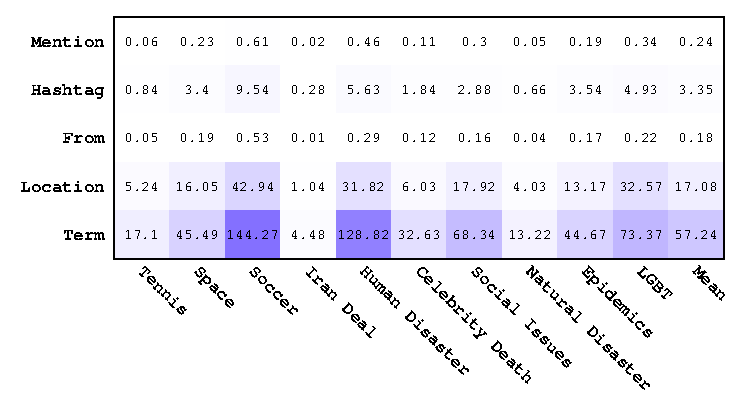
\includegraphics[width=\columnwidth]{images/avgMI.pdf}
\caption{Matrix of mean Mutual Information values (divided by $1E+10$ for different feature types vs. topics.  The last column is the average of mean values across all topics.)}
\label{fig:avgMI}
\end{figure}
%%%%%%%%%%%%%%%%%%%%%%%%%%%%%%%%%%%%%%%%%%%%%%%%%%%%%%%%%%%%%%%%%%%%%%%%%%%

%%%%%%%%%%%%%%%%%%%%%%%%%%%%%%%%%%%%%%%%%%%%%%%%%%%%%%%%%%%%%%%%%%
\begin{table*}[t!]
\centering
{
\resizebox{\textwidth}{!}{%
\begin{tabular}{|l|l|l|l|l|l|l|l|l|l|l|}
\hline
\textbf{Topics/Top10} & \textbf{NaturalDisaster} & \textbf{Epidemics} & \textbf{IranDeal} & \textbf{SocialIssues} & \textbf{LBGT} & \textbf{HumanDisaster} & \textbf{CelebrityDeath} & \textbf{Space} & \textbf{Tennis} & \textbf{Soccer} \\ \hline \hline
\textbf{From} & earthquake\_wo & changedecopine & mazandara & nsingerdebtpaid & eph4\_15 & ydumozyf & nmandelaquotes & daily\_astrodata & tracktennisnews & losangelessrh \\ \hline
\textbf{From} & earthalerts & drdaveanddee & hhadi119 & debtadvisoruk & mgdauber & syriatweeten & boiknox & freesolarleads & tennis\_result & shoetale \\ \hline
\textbf{From} & seelites & joinmentornetwk & 140iran & debt\_protect & stevendickinson & tintin1957 & jacanews & houston\_\_jobs & i\_roger\_federer & sport\_\_agent \\ \hline
\textbf{From} & globalfloodnews & followebola & setarehgan & negativeequityf & lileensvf1 & sirajsol & ewnreporter & star\_wars\_gifts & tennislessonnow & books\_you\_want \\ \hline
\textbf{From} & gcmcdrought & localnursejobs & akhgarshabaneh & dolphin\_ls & truckerbooman & rt3syria & paulretweet & lenautilus & kamranisbest & makeupbella \\ \hline \hline
\textbf{Hashtag} & earthquake & health & iran & ferguson & tcot & syria & rip & science & wimbledon & lfc \\ \hline
\textbf{Hashtag} & haiyan & uniteblue & irantalks & mikebrown & p2 & gaza & riprobinwilliams & starwars & usopen & worldcup \\ \hline
\textbf{Hashtag} & storm & ebola & rouhani & ericgarner & pjnet & isis & ripcorymonteith & houston & tennis & arsenal \\ \hline
\textbf{Hashtag} & tornado & healthcare & iranian & blacklivesmatter & uniteblue & israel & mandela & sun & nadal & worldcup2014 \\ \hline
\textbf{Hashtag} & prayforthephilippines & depression & no2rouhani & fergusondecision & teaparty & mh370 & nelsonmandela & sxsw & wimbledon2014 & halamadrid \\ \hline \hline
\textbf{Location} & philippines & usa & tehran & st.louis & usa & malaysia & southafrica & germany & london & liverpool \\ \hline
\textbf{Location} & ca & ncusa & u.s.a & mo & bordentown & palestine & johannesburg & roodepoort & uk & manchester \\ \hline
\textbf{Location} & india & garlandtx & nederland & usa & newjersey & syria & capetown & houston & india & london \\ \hline
\textbf{Location} & newdelhi & oh-sandiego & iran & dc & sweethomealabama! & israel & pretoria & austin & pakistan & nigeria \\ \hline
\textbf{Location} & newzealand & washington & globalcitizen & washington & aurora & london & durban & tx & islamabad & india \\ \hline \hline
\textbf{Mention} & oxfamgb & foxtramedia & 4freedominiran & deray & jjauthor & ifalasteen & nelsonmandela & bizarro\_chile & wimbledon & lfc \\ \hline
\textbf{Mention} & weatherchannel & obi\_obadike & iran\_policy & natedrug & 2anow & revolutionsyria & realpaulwalker & nasa & usopen & arsenal \\ \hline
\textbf{Mention} & redcross & who & hassanrouhani & antoniofrench & govchristie & drbasselabuward & robinwilliams & j\_ksen & andy\_murray & realmadriden \\ \hline
\textbf{Mention} & twcbreaking & obadike1 & un & bipartisanism & a5h0ka & mogaza & rememberrobin & jaredleto & serenawilliams & ussoccer \\ \hline
\textbf{Mention} & abc7 & c25kfree & statedept & theanonmessage & barackobama & palestinianism & tweetlikegiris & 30secondstomars & espntennis & mcfc \\ \hline \hline
\textbf{Term} & philippines & health & iran & police & obama & israel & robin & cnblue & murray & madrid \\ \hline
\textbf{Term} & donate & ebola & regime & protesters & gun & gaza & williams & movistar & tennis & goal \\ \hline
\textbf{Term} & typhoon & acrx & nuclear & officer & rights & israeli & nelson & enero & federer & cup \\ \hline
\textbf{Term} & affected & medical & iranian & protest & america & killed & mandela & ΍imperdible & djokovic & manchester \\ \hline
\textbf{Term} & relief & virus & resistance & cops & gop & children & cory & greet & nadal & match \\ \hline
\end{tabular}
}}
\caption{The top 5 features for each feature type and topic based on Mutual Information.}
\label{table:top10MItopicsLocations}
\end{table*}
%%%%%%%%%%%%%%%%%%%%%%%%%%%%%%%%%%%%%%%%%%%%%%%%%%%%%%%%%%%%%%%%%%

We now analyze the informativeness of our defined
features in Sec~\ref{sec:datasetStatistics} and the effect of their
attributes on learning targeted topical classifiers. 
We use Mutual Information (MI)~\cite{manning_ir} as our primary
metric for feature evaluation,   
where higher values for this metric indicate more informative features for the given topic.

We provide the mean Mutual Information
values for each feature across different topics in Fig.~\ref{fig:avgMI}.
The last column in Fig.~\ref{fig:avgMI} shows the
average of the mean Mutual Information for each feature type.  We observe
the following:
\begin{itemize}%[noitemsep] %nolistsep
\item The \textit{Term} and \textit{Location} features are the most informative features on average (despite class labels being \emph{Hashtags}).
\item The \textit{Location} feature provides second highest MI regarding the topics of \textit{HumanDisaster}, \textit{LBGT}, and \textit{Soccer} indicating that the content in these topics is heavily localized.
\item Looking at the overall average values, the order of informativeness of feature types appears to be the following: \textit{Term}, \textit{Location}, \textit{Hashtag}, \textit{Mention}, \textit{From}.
\end{itemize}

As anecdotal evidence to support these conclusions and provide additional insights regarding
the informativeness of each feature type, we refer to
Table~\ref{table:top10MItopicsLocations}, which displays the top five feature instances
for each feature type and topic.  Among many remarkable insights in this table, one key aspect  
we note is that the \emph{terms appear to be the most generic} (and hence most generalizable) features,
providing strong intuition as to why these features are informative over the two year time
span of our data.  The top \emph{locations are also highly relevant to most topics} indicating
the overall importance of these tweet features for identifying topical tweets.

\section*{Acknowledgments}
We thank Dan Nguyen for his help with data processing.

\bibliographystyle{aaai}
%\fontsize{9.0pt}{10.0pt}
%\selectfont
\bibliography{bibliography}

\end{document}
